\chapter[Introduction]{Introduction}
\label{cp:introduction}

{
	\parindent0pt
	This chapter introduces the fundamental concepts necessary to understand Molecular Dynamics (MD) simulations. We begin with a discussion of the motivation behind the general $n$-body problem and the goals of this thesis in \autoref{sec:motivation}.
	Afterwards, the components of a simple MD simulation loop are presented in \autoref{sec:md}. These include Newton’s laws of motion for providing the equations of particle trajectories, the Lennard-Jones potential as a model for pairwise interactions, and the Störmer-Verlet algorithms as numerical schemes for integrating the equations of motion.
}


\section{Motivation}
\label{sec:motivation}

The $n$-body problem is a foundational challenge of classical physics. It  concerns the interaction and movement of bodies, for example, the trajectories of masses in the solar system. At such astronomic scales, general relativity additionally introduces a high degree of complexity. Yet, even in classical Newtonian physics, the systems of equations tend to no longer be solvable by analytic means if $n>2$ bodies are involved, except for certain special cases. Hence, numerical algorithms have become essential in finding approximate solutions. \cite{Arnold1985}

With the advent of computer-based simulation, the feasibility of finding such numerical solutions to a $n$-body problem has increased significantly.
Over the past few decades, advances in high-performance computing (HPC) have further increased both scale and efficiency of such simulations, allowing for the modeling of large systems at unprecedented resolution. In 2017, for instance, the TianNu project simulated \num{2.97e12} particles on the Tianhe-2 supercomputer \cite{Emberson2017}.
These days, particle simulations have established themselves as indispensable tools across a wide range of scientific fields. Applications reach from drug design \cite{Hollingsworth2018} to plasma physics \cite{Verboncoeur2005} and materials science \cite{Parteli2016}. Two such applications are illustrated in \autoref{fig:particle_simulation_usecases}.

\begin{figure}
	\centering
	\begin{subfigure}[t]{0.45\textwidth}
		\vskip0pt
		\centering
		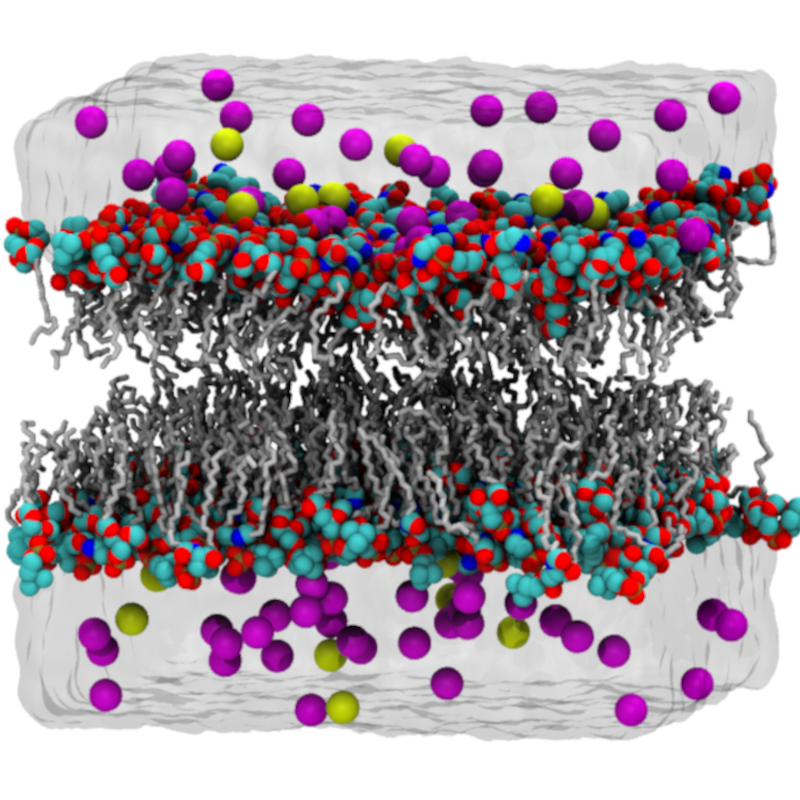
\includegraphics[width=0.6\textwidth]{applications/bilayer.png}
		\subcaption{Simulation of a lipid bilayer, representative for cell membranes. \cite{Vassiliev2025}}
	\end{subfigure}%
	\hspace{0.025\textwidth}
	\begin{subfigure}[t]{0.45\textwidth}
		\vskip0pt
		\centering
		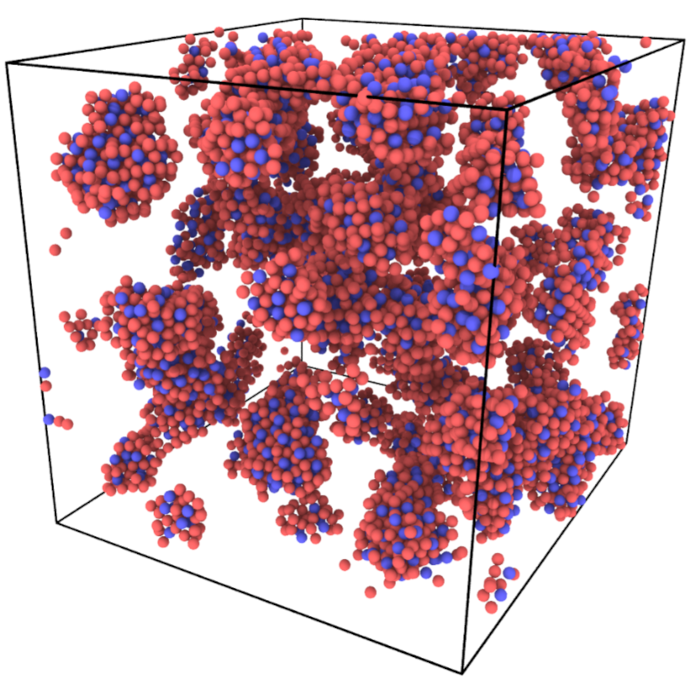
\includegraphics[width=0.6\textwidth]{applications/annealing.png}
		\subcaption{Simulation of crystal growth in metallic glass during annealing. \cite{Brink2017}}
	\end{subfigure}
	\caption{Real-world applications of MD simulations.}
	\label{fig:particle_simulation_usecases}
\end{figure}

One example of a software framework enabling $n$-body simulations is the AutoPas library \cite{Gratl2019}. Its internal mechanisms will be discussed in detail in \autoref{cp:autopas}; for the motivation of this thesis it suffices to know, that AutoPas seeks to dynamically select optimal algorithmic configurations without requiring expert knowledge during setup (\enquote{autotuning}).

To achieve this, so-called tuning phases are initiated at fixed intervals. During each tuning phase, different configurations are sampled for a predetermined number of iterations, after which the best performing configuration is selected to simulate the remaining iterations until the next tuning phase. Naturally, these static intervals do not necessarily align with the points at which it would be most advantageous to switch configurations. Consider a scenario, in which the optimal configuration changes rapidly in the beginning, but stabilizes and settles into an equilibrium later on. Having one uniform static interval, it would be either too short --- resulting in unnecessary tuning phases during equilibrium, or too long --- resulting in suboptimal performance in the early phase.
This thesis proposes a method to solve this problem by dynamically initiating tuning phases based on live simulation data.


\section{Molecular Dynamics}
\label{sec:md}
% quantum behaviour
Molecular Dynamics (MD) simulation is one method of solving the classical $n$-body problem on the molecular level. On that scale, the interactions between atoms are subject to the of laws quantum mechanics, in particular the Schrödinger equation. That equation, however, is unsuitable for the simulation of larger systems due to its complexity as it is a partial differential equation.

Therefore, simplifications such as the Born-Oppenheimer approximation have to be employed. This approximation is based on the fact that the nuclei of atoms have much greater mass than the electrons surrounding them. Under the additional assumption, that the nuclei can be considered as static, relative to the movements of the electrons, we can separate the Schrödinger equation into two parts coupled by an interaction potential. Using further simplifications, we obtain \eqref{eq:born_oppenheimer}, which directly corresponds to the classical laws of motion as stated by Newton (cf. \autoref{sec:newton}). In this equation, $\vb p_i(t), \vb a_i(t), m_i, V\left(\vb p_i(t)\right)$ are the position, acceleration, mass and potential acting on a particle $i$ at time $t$. \cite{Born1927, Voorhis2005, Griebel2007} 

\begin{equation}
	m_i\vb a_i(t) = -\nabla_{\vb p_i} V\left(\vb p(t)\right)\label{eq:born_oppenheimer}
\end{equation}

The simplest interatomic potentials one could apply here describe the interactions between only two particles, such as the Gravitational, Lennard-Jones or Coulomb potentials \cite{Griebel2007}.
Considering the formula presented in \eqref{eq:born_oppenheimer}, the main MD simulation loop is rather simple. One iteration of said loop consists of calculating the forces between particles and integrating the equations of motion. These two steps are repeated until an equilibrium is reached, at which point any desired measurements can be taken. \cite{Frenkel2002}





\subsection{Newton's Laws of Motion}
\label{sec:newton}
As referred to before, Newton's laws of motion can be applied to MD simulation in approximating particle behavior. These well-known laws of classical mechanics are as follows. \cite{Newton1934}
\begin{enumerate}[label=\Roman*.]
	\item \textit{Every object perseveres in its state of rest, or of uniform motion in a right line, unless it is compelled to change that state by forces impressed thereon.}

	      In other words, if the net force on any body is zero, its velocity is constant.
	\item \textit{The alteration of motion is ever proportional to the motive force impressed; and is made in the direction of the right line in which that force is impressed.}

	      In other words, $F=m\cdot a$.
	\item \textit{To every action there is always opposed an equal reaction: or, the mutual actions of two bodies upon each other are always equal, and directed to contrary parts.}

	      In other words, if one body exerts force $F_a$ on another body, than the latter exerts force $F_b=-F_a$ on the first body.
\end{enumerate}

The second law is particularly significant, as it allows to compute the trajectories of particles based on the forces acting upon them. The third law, while secondary in dynamics, is useful especially regarding optimizations: for pairwise interactions, any force needs to be evaluated only once, since the second particle experiences a force of the same magnitude in opposed direction. \cite{Gratl2021}

\subsection{Lennard-Jones Potential}
\label{sec:lj_potential}
Simulating all pairwise interactions between atoms has complexity $\mathcal{O}\left(n^2\right)$. To reduce this complexity, most MD simulations restrict themselves to short-range interactions. As the forces of these interactions are negligible if the interacting particles are far apart, a cutoff-radius $r_c$ can be introduced, beyond which the forces can be assumed negligible. This significantly reduces the computational complexity, as only the interactions between close neighbors have to be computed. Under optimal conditions, the number of interaction computations can be reduced to $\mathcal{O}\left(n\right)$. \cite{Gratl2021}

The Lennard-Jones (LJ) potential is one such short-range interaction potential that acts on pairs of particles. It is based on empirical data and provides a sufficiently good approximation, such that macroscopic effects can be derived from simulating interactions at a molecular level.
It is most frequently used in the form of the 12-6 potential as defined in \eqref{eq:lj_12_6}.

\begin{equation}
	V_{\text{LJ}}(r)=4\varepsilon\left[\left(\frac{\sigma}{r}\right)^{12}-\left(\frac{\sigma}{r}\right)^{6}\right]\label{eq:lj_12_6}
\end{equation}

In this equation, $r$ is the distance between the two particles, $\varepsilon$ the interaction strength and $\sigma$ the distance at which the potential signs change (zero-crossing). Parameters $\varepsilon, \sigma$ are dependent on the simulation context, e.g. the material which ought to be simulated. The potential function is illustrated in \autoref{fig:lj_graph}. \cite{Wang2020, Lenhard2024}


\begin{figure}[htpb]
	\centering
	\begin{tikzpicture}
		\begin{axis}[height=0.4\textwidth, width=0.6\textwidth,
			xmin = 0.75,
			xmax = 3.25,
			ymin = -1.25,
			ymax = 2.25,
			xlabel={Distance $r$ between Particles},
			ylabel={Potential $V_{\text{LJ}}$},
			xtick={{2^(1/6)},1.5,2,2.5,3},
			xticklabels={$r_\text{min}$,1.5$\sigma$,2$\sigma$,2.5$\sigma$,3$\sigma$},
			ytick={-1, 0, 1, 2},
			yticklabels={$-\varepsilon$,0,$\varepsilon$,2$\varepsilon$},
			clip=false]
			\addplot [
				color=chaptertumblue, very thick,
				domain=0.95:3,
				samples=400,
			]
			{4*((1/x)^(12) - (1/x)^6)};
			\draw[black!80] (axis cs:0.75,0) -- (axis cs:3.25,0);
			\draw[black!80] (axis cs:{2^(1/6)},2.25) -- (axis cs:{2^(1/6)},-1.25);
			\draw[black!80, dashed] (axis cs:0.75,-1) -- (axis cs:{2^(1/6)},-1);
			
			\draw[black!80, dashed] (axis cs:2.5,-1.25) -- (axis cs:2.5,2.25);
			\node[anchor=south west, align=left] at (axis cs:2.5, 0) {$r_c$};
			
			
			\draw [decorate,decoration={brace, amplitude=1ex, raise=0.5ex}] (axis cs:0.75,2.25) -- (axis cs:{2^(1/6)-0.0125},2.25) node[midway, yshift=2.5ex, , text depth=0.5em]{Repulsion};
			\draw [decorate,decoration={brace, amplitude=1ex, raise=0.5ex}] (axis cs:{2^(1/6)+0.0125},2.25) -- (axis cs:3.25,2.25) node[midway, yshift=2.5ex, text depth=0.5em]{Attraction};
		\end{axis}
	\end{tikzpicture}
	\caption{An illustration of the 12-6 LJ potential well, with the minimum of $-\varepsilon$ at $r_\text{min}=\sigma\sqrt[6]{2}$, zero-crossing at $\sigma$ and cutoff radius $r_c$. The figure is based on Lenhard et al. \cite{Lenhard2024}}
	\label{fig:lj_graph}
\end{figure}



\subsection{Störmer-Verlet Algorithm}
\label{sec:stoermer_verlet}
Using LJ potentials and Newton's laws of motion, we can construct a system of ordinary differential equations. Solving them analytically is practically infeasible for large systems, therefore numeric methods have to be used in approximating a solution, as stated before.

The Störmer-Verlet algorithm is one such numeric method for solving these systems.
With $\vb p_i(t), \vb v_i(t), \vb a_i(t), m_i, \vb F_i(t)$ as the position, velocity, acceleration, mass and force acting on a particle $i$ at time $t$, we can derive the algorithm by the summation of Taylor expansions. First, we deduce the position of particle $i$ at time $t+\delta t$, as in \eqref{eq:pos_taylor_forward}. Secondly, we take a backwards step to $t-\delta t$, as in \eqref{eq:pos_taylor_backward}.
\begin{equation}
	\vb p_i(t+\delta t) = \vb p_i(t)+\delta t\dot{\vb p}_i(t)+\frac{1}{2}\delta t^2\ddot{\vb p}_i(t)+\frac{1}{6}\delta t^3\dddot{\vb p}_i(t)+\mathcal{O}(\delta t^4)\label{eq:pos_taylor_forward}
\end{equation}
\begin{equation}
	\vb p_i(t-\delta t) = \vb p_i(t)-\delta t\dot{\vb p}_i(t)+\frac{1}{2}\delta t^2\ddot{\vb p}_i(t)-\frac{1}{6}\delta t^3\dddot{\vb p}_i(t)+\mathcal{O}(\delta t^4)\label{eq:pos_taylor_backward}
\end{equation}

By adding both \eqref{eq:pos_taylor_forward} and \eqref{eq:pos_taylor_backward} and reordering terms, we conclude \eqref{eq:pos_verlet}.
\begin{equation}
\vb p_i(t+\delta t) = 2\vb p_i(t) - \vb p_i(t-\delta t) + \delta t^2\ddot{\vb p}_i(t) + \mathcal{O}(\delta t^4)\label{eq:pos_verlet}
\end{equation}

As the second derivative of the position $\vb p_i(t)$ is the acceleration $\vb a_i(t)$, we can express \eqref{eq:pos_verlet} as \eqref{eq:acc_verlet}. Where, by Newton's second law, $\vb a_i(t) = \frac{\vb F_i(t)}{m_i}$.
\begin{equation}
	\vb p_i(t+\delta t) = 2\vb p_i(t) - \vb p_i(t-\delta t) + \delta t^2{\vb a}_i(t) + \mathcal{O}(\delta t^4)\label{eq:acc_verlet}
\end{equation}

Using this result, we could already calculate the velocities of the individual particles. However, there are some drawbacks, e.g., high error propagation \cite{Fulst2013}. A more exact and efficient approach, sometimes referred to as the Velocity-Verlet algorithm, can be derived similarly.
For that, considering \eqref{eq:velocity}, we can rearrange and substitute into \eqref{eq:pos_verlet} to conclude \eqref{eq:verlet_pos2} and finally \eqref{eq:verlet_vel}.
\begin{equation}
	\vb v_i(t) = \frac{\vb p_i(t+\delta t) -\vb p_i(t-\delta t)}{2\delta t} \rightsquigarrow \vb p_i(t-\delta t)= \vb p_i(t+\delta t)-2\delta t \vb v_i(t) \label{eq:velocity}
\end{equation}

\begin{equation}
	\vb p_i(t+\delta t) = \vb p_i(t) +\delta t \vb v_i(t) + \frac{\delta t^2}{2}{\vb a}_i(t) + \mathcal{O}(\delta t^4) \label{eq:verlet_pos2}
\end{equation}
\begin{equation}
	\vb v_i(t+\delta t) = \vb v_i(t)+\frac{\delta t}{2}\left[\vb a_i(t)+ \vb a_i(t+\delta t)\right] + \mathcal{O}(\delta t^4) \label{eq:verlet_vel}
\end{equation}
Because of the aforementioned improved properties of this method, it is often preferred in MD simulations. \cite{Fulst2013, Leimkuhler2005, Hairer2003}





